% !TEX root = ../../main.tex
\section{Other conic sections}
\label{sec:other-conics}

So far we have focused on the elliptic (bound) case. In the same inverse-square central-force setting, the remaining conic trajectories are the parabola (threshold case) and the hyperbola (unbound case), together with one degenerate limit discussed first.

\subsection{Rectilinear motion as a degenerate conic limit}
\label{subsec:strange-line}

This extreme limit corresponds to rectilinear motion. It can be viewed as a collapsed ellipse with $a=c$ and $b=0$, i.e., a degenerate conic with zero areal speed about the force center. That case is outside the present scope: here we use nondegenerate conic geometry together with nonzero constant areal speed to solve the inverse problem. For a straight-line orbit, many different centripetal laws can produce the same geometric path, and the real task is to determine the time parametrization of motion along the line. We therefore omit this case, though Newton discusses it in detail in the \emph{Principia} using geometric parametrizations.

\subsection{Hyperbola}
\label{subsec:hyperbola}

For an inverse-square central force, hyperbolic trajectories correspond to unbound motion: the point mass comes in from infinity and escapes back to infinity, with the force center located at a focus of the hyperbola.

See \Cref{fig:hyperbola} for the auxiliary-circle construction used to carry out the same inverse-square argument in the hyperbola case.
\begin{figure}[!t]
  \centering
  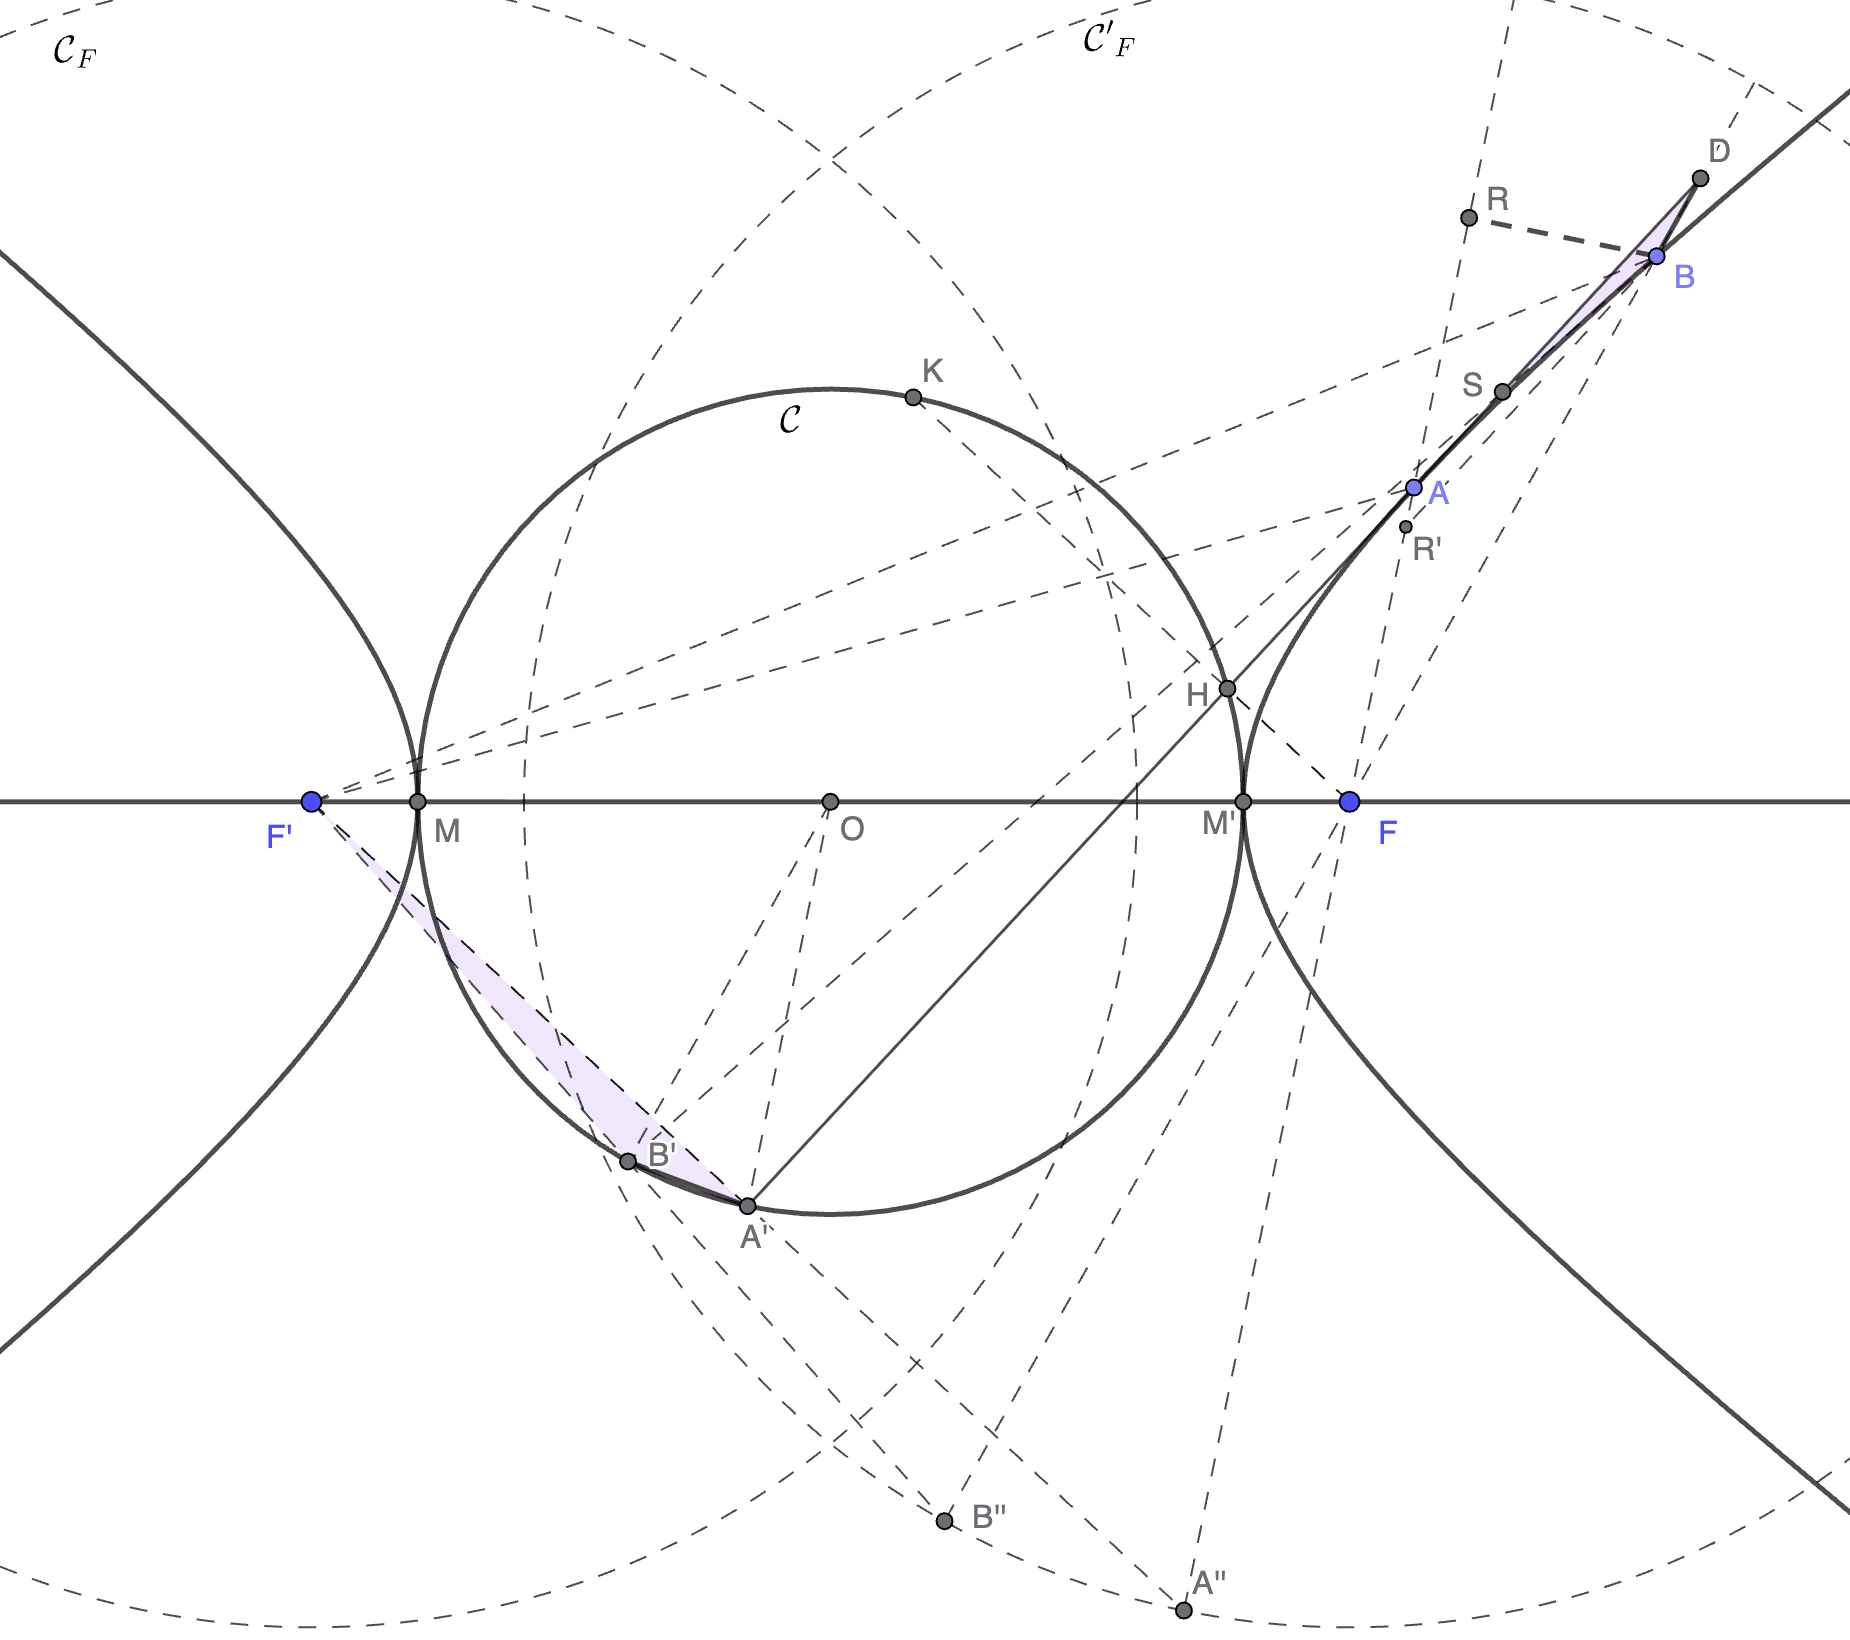
\includegraphics[width=0.9\linewidth]{assets/images/hyperbola.png}
  \caption{Auxiliary-circle construction for the hyperbola case.}
  \label{fig:hyperbola}
\end{figure}
In this hyperbola setup, one may again view the auxiliary circle $\mathcal C$ as providing a convenient geometric proxy for the (circular) hodograph, with $F'$ taken as the velocity origin.
As in the \Cref{fig:proof2-ellipse} for elliptic case, this proxy picture must be rotated by $90^\circ$ to match the correct direction of the velocity vector in the hodograph construction.

Likewise, the directrix circle $\mathcal{C}_{F'}$ may be regarded as a $2\times$ scaling of the auxiliary circle $\mathcal C$ with scaling center $F'$; consequently it can also be interpreted as a scaled version of the hodograph, again up to the same $90^\circ$ rotation.

The same key product identity (\Cref{lem:product-identity}) also holds in this hyperbola setting, though processed differently:
\begin{equation}
  F'\!A'\cdot FH = FH\cdot FK = F\!M'\cdot FM = (c-a)(c+a)=c^2-a^2=b^2,
\end{equation}
using the same tangent/intercept relations (here $c=OF$ and $a^2=b^2+c^2$).

Similarly, in the analogue of inverse problem Proof~2 the computation is again driven by the same pair of similar triangles $\triangle F'\!A'B'$ and $\triangle SDB$.

There is also a ``swapped-focus'' situation leading to the same right-branch hyperbola: instead of an attractive (centripetal) force toward $F$, one may consider a centrifugal force directed away from $F'$ acting on the particle as it moves from $A$ to $B$.
In that case to carry out the proof, the roles of $F$ and $F'$ are interchanged, and the point $R$ is dropped onto the extension of the new line $FA$.
The points $H$ and $A'$ also exchange roles, $B'$ moves to the opposite side of the auxiliary circle $\mathcal C$, and $D$ becomes the intersection of the tangent line at $A$ with the new line $FB$ (namely, $F'B$ as in \Cref{fig:hyperbola}). Readers should be able to construct the modified plot accordingly without difficulty, and the proof then follows in exactly the same way.

So once \Cref{fig:hyperbola} is in place, the remaining steps corresponding to our Proofs~2 and~3 for the hyperbola follow with only minor, mostly notational, changes. In particular, once the hyperbola geometry yields a constant limit for $BD/BR^2$, \Cref{lem:bd-over-br2} gives the inverse-square form directly.

\subsection{Parabola}
\label{subsec:parabola}

\subsubsection{Parabola as a limiting conic and hodograph setup}
\label{subsubsec:parabola-general}

The parabolic trajectory is the boundary between bound (elliptic) and unbound (hyperbolic) motion.
It is also distinguished geometrically as the conic section obtained when the cutting plane is parallel to a generating edge of the cone.

One can also view a parabola as a limiting ellipse in which $a,c\to\infty$ while $(a\!-\!c)$ stays finite.
Indeed, since $p=b^2/a=(a+c)(a-c)/a$, in this limit one has $p\to 2(a-c)$.
It is therefore natural to parametrize the parabola by setting $a-c$ as a single parameter $a'$, so that $p=2a'$, called(??). From this perspective, the auxiliary circle degenerates to the tangent line at the vertex of the parabola, for at the vertex this infinit-radius circle is a line perpendicular to the symmetry axis $AF$ (with $F$ the remaining focus).

This is consistent with the polar form: the eccentricity satisfies $e=c/a=1$ for a parabola. One can similarly think of the parabola as an approximation/limit of hyperbolas as $a,c\to \infty$ while keeping $(c\!-a)$ constant.

As the eccentricity of an ellipse tends to 1, the second focus recedes to $\infty$ along the axis; in the limit it becomes a remote focus. Hence the “directrix circle” construction from the ellipse case no longer survives as a literal circle centered at the observed focus.
Yet the effect of that construction does survive: a circle of infinite radius, centered at the remote focus, degenerates into a straight line perpendicular to the axis—namely the parabola’s directrix. In this limiting viewpoint the directrix may be regarded as the remnant of the former directrix circle, positioned so that it meets the axis
$AF$ at a point symmetrically placed with respect to the vertex
$A$ (in the same sense as in the elliptical construction). So while an ellipse and a hyperbola each have two directrix circles and two directrix lines, a parabola has only one observable directrix ``circle'' that's a directrix line while the other would be at infinity that's not meaningful to consider. Furthermore, this circle degenerates to the same line. The directrix line is joining the jamor axis at $2a-(a+c) = a-c=a'$ away from the vertex, so it is located on the opposite side of the focus with equal distance to the vertex.

However, we will also show that a parabola still admits several natural associated circles that encode useful geometry. In particular, although the earlier auxiliary circle and directrix circle have both degenerated into a line, one may still construct rotated hodograph circle(s) with various scalings and velocity origin, similar to what we have done for the ellipse and hyperbola, which remains genuinely circular and retains the kinematic/geometric information needed for our proofs. Since parabola has only one degree of freedom $a'$, there are more relationships among angles and distances than in the generic conic sections. Generally parabola treatment is considered a simpler special case of the more general conic sections, but in some ways it is more subtle and requires special care to handle, as we will see in the proofs below.

In this section we show that the analogues of inverse problem Proofs~2 and~3 from the ellipse case also hold for the parabola, with some special care.
We recommend reading Newton-style arguments (in the 1687 tradition), such as the historical collection of various properties of the parabola in \href{https://doi.org/10.5539/apr.v11n2p30}{\cite{stavek2019newtonsparabola}}.
A much clearer explanation of the hodograph for the parabolic case is given by Derbes (2001) \cite{derbes2001reinventing}, which uses the circle centered at the focus $F$ with radius $2a'$ which further showed the Maxwell (1877)/Hamilton (1847) hodograph proof for the inverse problem also extends naturally to the parabola.

\subsubsection{Parabola variant of inverse problem Proof 2: a constant \texorpdfstring{$BR^2/BD$}{BR squared over BD}}
\label{subsubsec:parabola-proof2}

\begin{figure}[t]
  \centering
  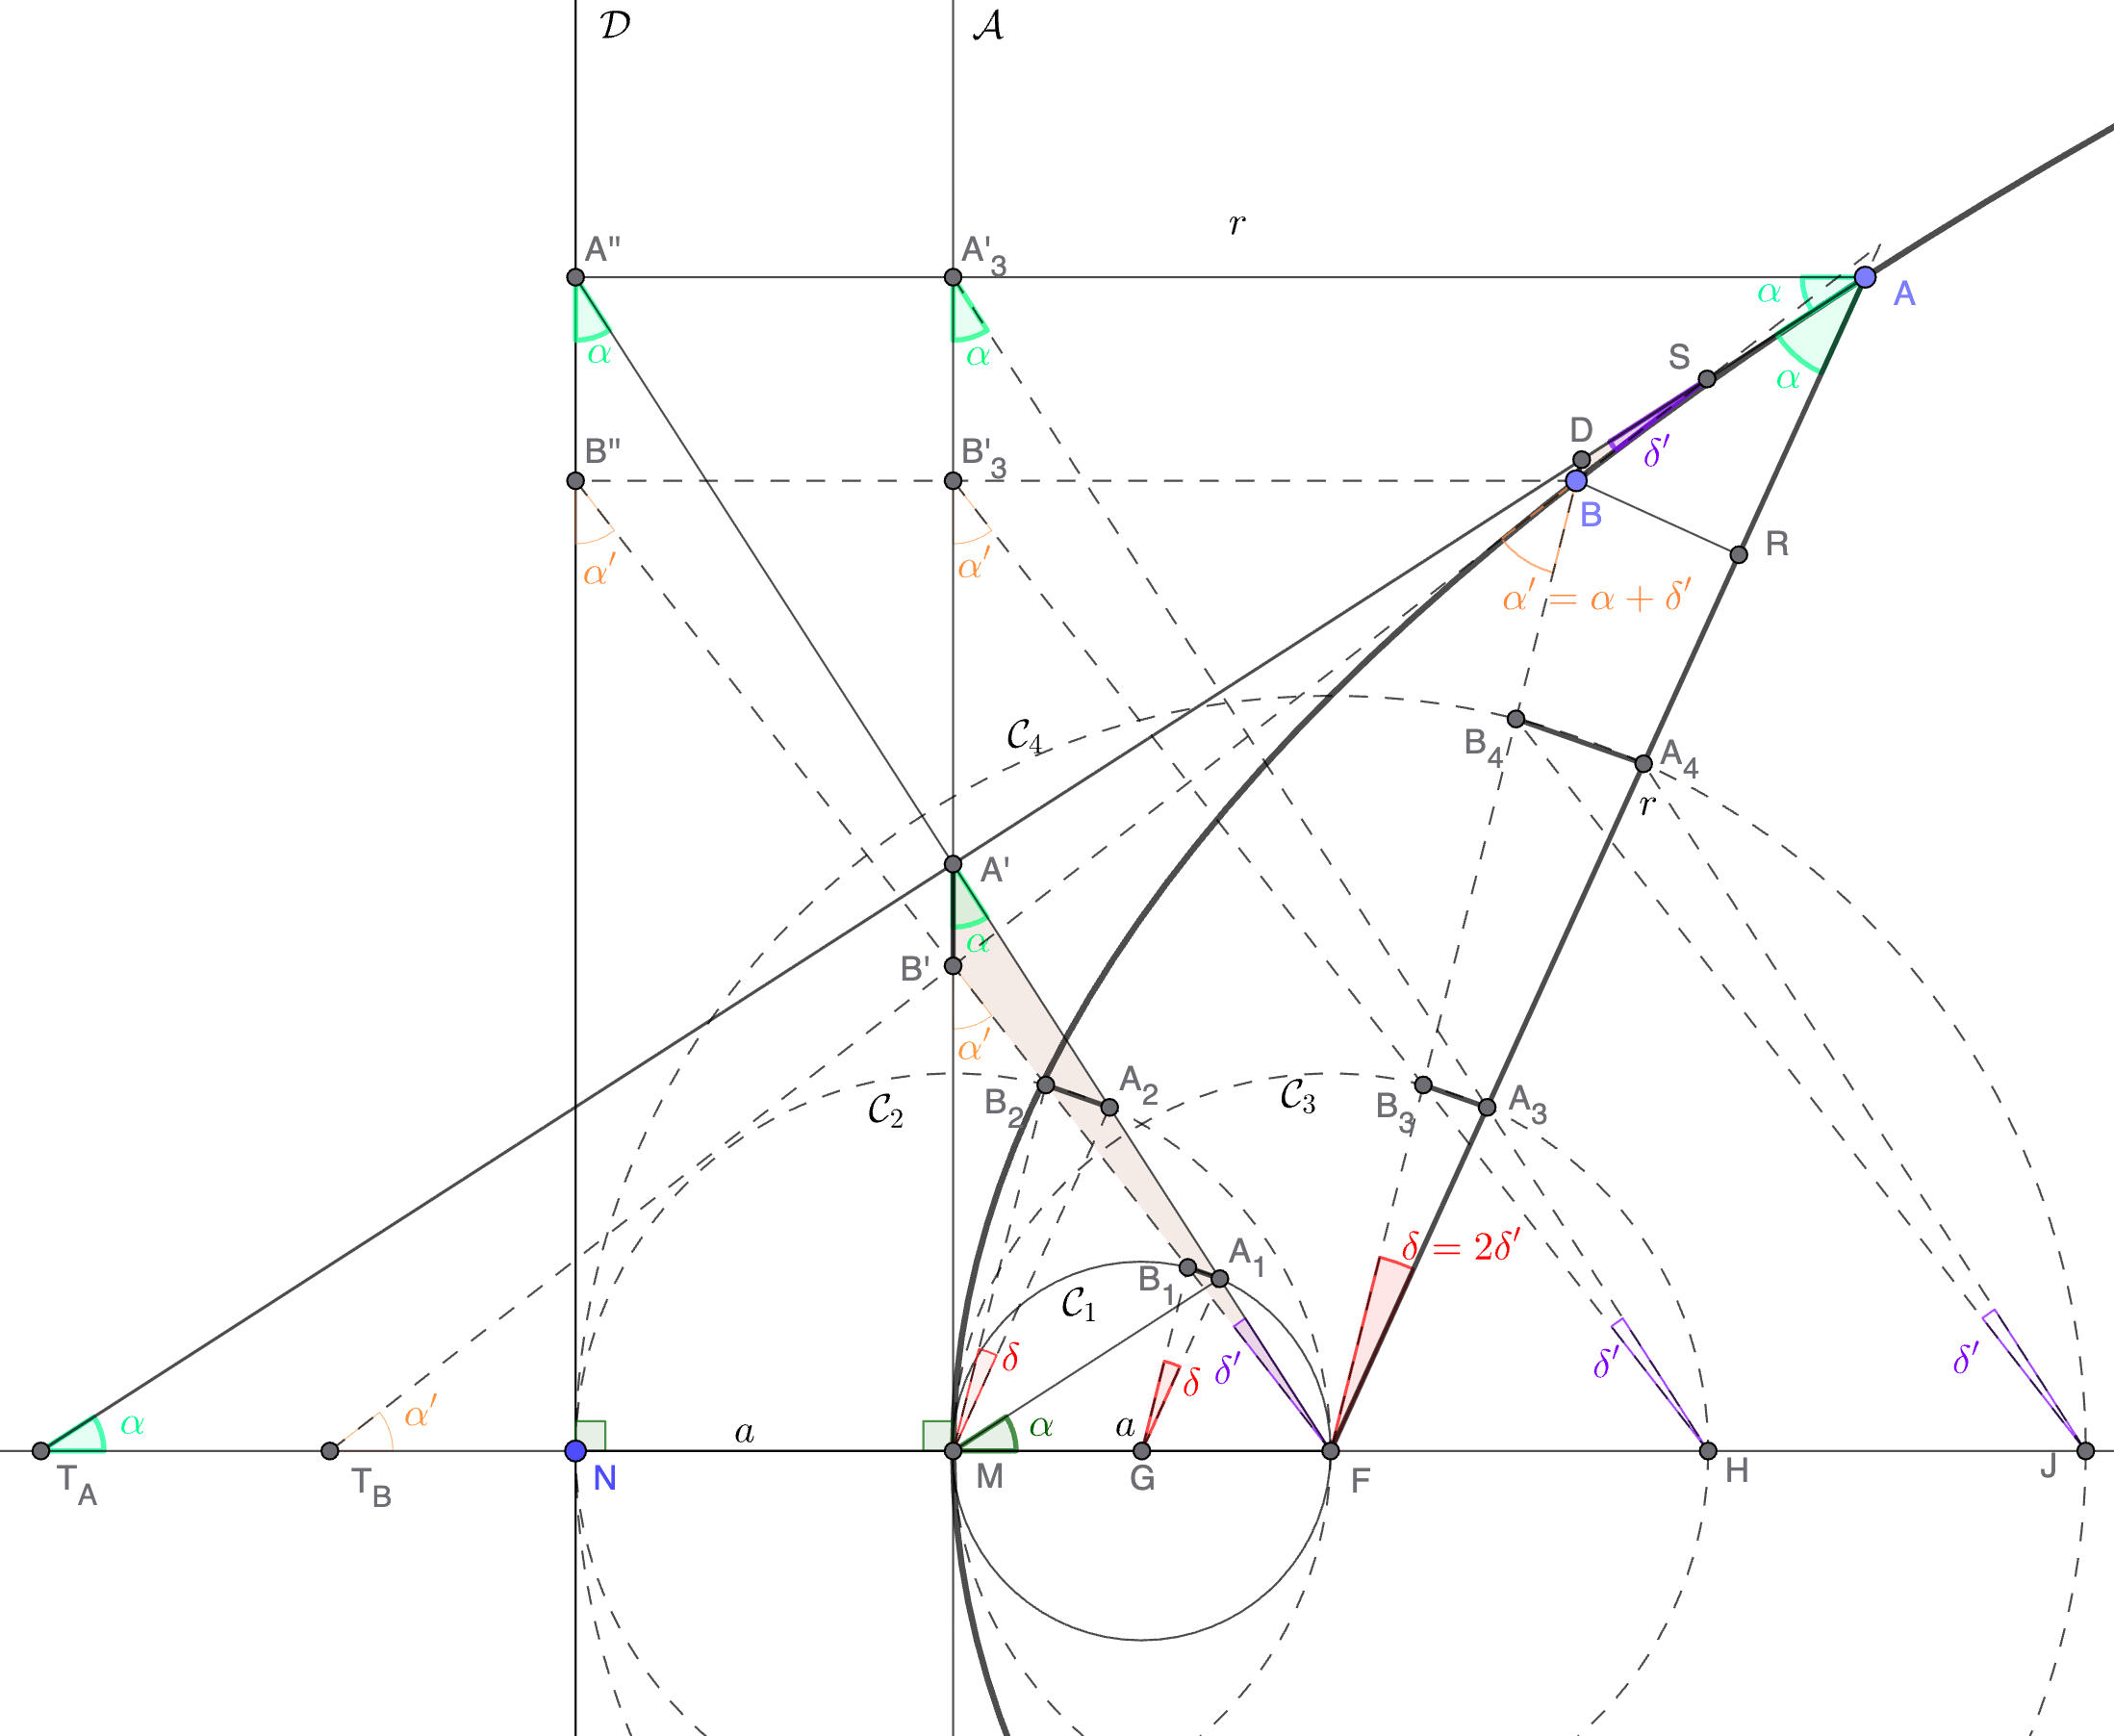
\includegraphics[width=\linewidth]{assets/images/parabola.png}
  \caption{Parabola construction used in Section~\ref{subsec:parabola} (parabola analogue of inverse problem Proof~2).}
  \label{fig:parabola-proof2}
\end{figure}

This is the parabola analogue of inverse problem Proof~2 in the auxiliary-circle style. For convenience in the rest of the discussion we will simply use $a$ instead of $a'$ to denote the parabola parameter, so that the semi-latus rectum is $p=2a$.

\begin{proposition}[Parabola variant of inverse problem Proof~2]
\label[proposition]{prop:parabola-br2-over-bd}
In the parabolic construction (notation matching the ellipse case), as $B\to A$ one has
\begin{equation}
  \lim_{B\to A}\frac{BR^2}{BD}=4a,
\end{equation}
where $a$ is the parabola parameter (so the semi-latus rectum is $p=2a$).
\end{proposition}

\begin{proof}
As $B\to A$ (small angles $\delta,\delta'\to 0$), similar triangles in the figure give
\[
  \frac{A'B'}{BD}=\frac{B'F}{DS}\sim \frac{2\,B'F}{DA}.
  \qquad\text{(1)}
\]
Resolve the ratio with the common angle $\alpha$:
\[
  \frac{B'F}{DA}
  =
  \frac{B'F\sin\alpha}{DA\sin\alpha}
  \sim \frac{a}{BR}.
  \qquad\text{(2)}
\]
since $DA\sin\alpha\sim BR$ and $B'F\sin\alpha=a$. Substituting (2) into (1),
\[
  \frac{A'B'}{BD}\sim \frac{2a}{BR},
  \qquad\text{so}\qquad
  BD\sim \frac{A'B'\,BR}{2a}.
  \qquad\text{(3)}
\]
Also $A'B'\sim r\delta'$ and $BR=2r\delta'$, hence $A'B'\sim \tfrac12 BR$. Therefore
\[
  BD\sim \frac{(\tfrac12 BR)\,BR}{2a}=\frac{BR^2}{4a},
\]
so $\dfrac{BR^2}{BD}\to 4a$.

An equivalent shortcut (as suggested) is to use $\triangle SDB\sim\triangle FDS$, giving
\[
  DS^2\sim DB\cdot FS,\qquad DB\sim \frac{DS^2}{FS}.
\]
With $DS=\tfrac12 AD$ and the same $\alpha$-projection relations, one again obtains
\[
  DB\sim \frac{BR^2}{4a},
\]
hence the same limit $\dfrac{BR^2}{BD}\to 4a$.
\end{proof}

\Cref{prop:parabola-br2-over-bd} is the inverse-problem parabolic counterpart of \eqref{eq:proof2-bd-br2} in the elliptic setting. Since
\[
  \frac{BR^2}{BD}\to 4a
  \quad\Longleftrightarrow\quad
  \frac{BD}{BR^2}\to \frac{1}{4a},
\]
\Cref{lem:bd-over-br2} gives
\[
  a_F=\frac{2L^2}{r^2}\cdot\frac{1}{4a}
  =\frac{L^2}{2a}\,\frac{1}{r^2}
  =\frac{L^2}{p}\,\frac{1}{r^2}
  \qquad (p=2a),
\]
and therefore
\[
  \mathbf a_F(r)=-\mu\,\frac{\mathbf r}{r^3},
  \qquad
  \text{i.e. }\mathbf a_F(r)=-\frac{\mu}{r^2}\,\hat r,
  \qquad
  \mu=\frac{L^2}{p}
  \quad (p=2a).
\]

\subsubsection{Parabola variant of inverse problem Proof 3: direct hodograph-circle use}
\label{subsubsec:parabola-proof3}

\begin{proposition}[Parabola variant of inverse problem Proof~3]
Using the hodograph-circle quantities in \Cref{fig:parabola-proof2}, one again obtains
\[
  a_F=\frac{L^2}{p}\frac{1}{r^2},
  \qquad
  \mathbf a_F(r)=-\mu\,\frac{\mathbf r}{r^3},
  \qquad
  \mu=\frac{L^2}{p},
  \quad (p=2a).
\]
\end{proposition}

\begin{proof}
In the parabola construction, let $A_1,B_1$ be the corresponding points on the hodograph-related circle. Since $MA_1\perp FA$,
\[
  FA_1\cdot FA' = FM^2 = a^2.
\]
Using the areal-rate relation in the same form as before,
\[
  v\cdot FA' = L
  \quad\Longrightarrow\quad
  FA_1=\frac{v\,a^2}{L}.
\]
For a neighboring point $B$, this gives
\[
  A_1B_1=\Delta(FA_1)=\frac{a^2}{L}\,\Delta v.
\]
From the local parabola similarity in this construction,
\[
  DB=\frac{2r}{a}\,A_1B_1
  =\frac{2ra}{L}\,\Delta v.
\]
Also, from the same local area step,
\[
  DB\cdot r = L\,\Delta t.
\]
Hence
\[
  \frac{2ra}{L}\,\Delta v\cdot r=L\,\Delta t
  \quad\Longrightarrow\quad
  a_F=\frac{\Delta v}{\Delta t}
  =\frac{L^2}{2a}\frac{1}{r^2}
  =\frac{L^2}{p}\frac{1}{r^2},
  \qquad (p=2a).
\]
Therefore
\[
  \mathbf a_F(r)=-\mu\,\frac{\mathbf r}{r^3},
  \qquad
  \text{i.e. }\mathbf a_F(r)=-\frac{\mu}{r^2}\,\hat r,
  \qquad
  \mu=\frac{L^2}{p}.
\]
\end{proof}
